\subsection{子領域における地形の取り扱い} \label{subsec:nest_topo}
%------------------------------------------------------
ネスティング実験を行う際、親領域と子領域間で空間解像度が異なるため、
一般的には地形の解像度も異なる。
\scalerm では、
子領域の緩和領域内で不整合が発生する
可能性がある。
緩和領域内は親領域の計算結果を用いて一部の変数を緩和していくが、地形の表現性が異なる
ことで、子領域にとっては正しくない値へ引きずられる可能性がある。
例えば、子領域では斜面上の小さな谷として
表現されている地形が、親領域では格子間隔が大きすぎて
谷がなくスムーズな斜面として表現される場合が考えられる。

こういった不整合を無くすために、緩和領域では親領域の地形を用い、内側領域では子領域自身の地形を用いる
「地形コピー」の機能が実装されている。この機能を使えば、図\ref{fig_topocopy}に示すように緩和領域は完全に
親領域に一致する地形で、内側に移る地形遷移領域内では親領域と子領域のミックス、それより内側では完全に
子領域の地形という設定を構築することができる。以降、その設定方法と実行手順を説明する。


ここで説明する地形コピーの設定を記述した\verb|pp.d0*.conf|ファイルがチュートリアルディレクトリ
\verb|${Tutorial_dir}/real/sample/online_nesting|に置いてあるので、
説明を読み進める上で参考にしてもらいたい。

\begin{figure}[tb]
\begin{center}
  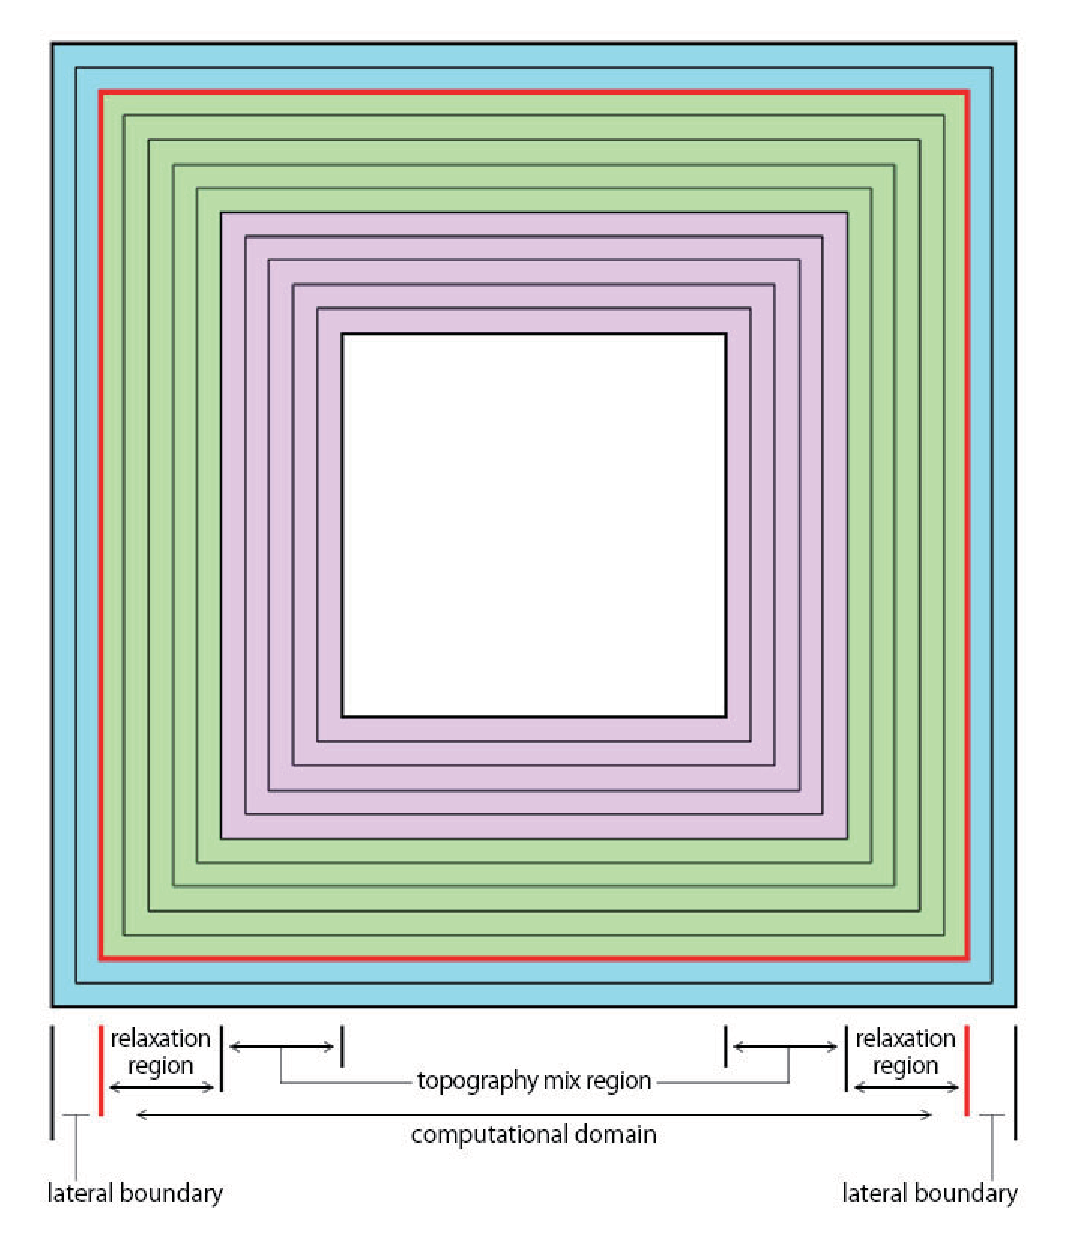
\includegraphics[width=0.4\hsize]{./figure/topo_copy.eps}\\
  \caption{地形コピーを適用した子領域の地形データ水平分布. 最外の水色の2格子(\texttt{HALO}の数。水平差分スキームによって異る)は側面境界で、それより内側の赤色の線で
           囲われた領域が計算領域である。緑色の部分が緩和領域、桃色の部分が地形遷移領域、そして最内の白色の
           部分が子領域の地形をもつ領域である。地形遷移領域では外側から内側にかけて徐々に親領域の地形データから
           子領域の地形データへ遷移する。}
  \label{fig_topocopy}
\end{center}
\end{figure}

まず親領域の``pp.d01.conf''ファイルを編集して、計算領域の大きさを子領域へ伝えるために緯度経度カタログ
ファイルを出力するように設定する。具体的には、下記の記述を``pp.d01.conf''ファイルに追記する。\\

\noindent {\small {\gt
\ovalbox{
\begin{tabularx}{140mm}{l}
\verb|&PARAM_DOMAIN_CATALOGUE| \\
\verb| DOMAIN_CATALOGUE_FNAME  = "latlon_domain_catalogue.txt",| \\
\verb| DOMAIN_CATALOGUE_OUTPUT = .true.,| \\
\verb|/| \\
\end{tabularx}
}}}\\

\noindent その他の設定項目は通常通りで良い。編集ができたら親領域の地形データ作成を実行する(つまり、
scale-rm\_ppを実行する)。ここで、出力データは、``topo\_d01.pe***.nc''というファイル名で保存されていると
想定する。次に、子領域の``pp.d02.conf''ファイルを編集する。\\

\noindent {\small {\gt
\ovalbox{
\begin{tabularx}{140mm}{l}
\verb|&PARAM_CNVTOPO| \\
\verb|     〜 中略 〜|\\
\verb| CNVTOPO_copy_parent     = .true.,| \\
\verb|/| \\
 \\
\verb|&PARAM_COPYTOPO| \\
\verb| COPYTOPO_IN_BASENAME   = "topo_d01",| \\
\verb| COPYTOPO_ENTIRE_REGION = .false.,| \\
\verb| COPYTOPO_LINEAR_H      = .true.,| \\
\verb|/| \\
 \\
\verb|&PARAM_NEST| \\
\verb| USE_NESTING               = .true.,| \\
\verb| OFFLINE                   = .true.,| \\
\verb| OFFLINE_PARENT_PRC_NUM_X  = 4,| \\
\verb| OFFLINE_PARENT_PRC_NUM_Y  = 4,| \\
\verb| OFFLINE_PARENT_KMAX       = 35,| \\
\verb| OFFLINE_PARENT_IMAX       = 40,| \\
\verb| OFFLINE_PARENT_JMAX       = 40,| \\
\verb| OFFLINE_PARENT_LKMAX      = 5,| \\
\verb| LATLON_CATALOGUE_FNAME    = "latlon_domain_catalogue.txt",| \\
\verb|/| \\
\end{tabularx}
}}}\\

\noindent 
地形コピーを用いるには、もともと設定ファイルにある\namelist{PARAM_CNVTOPO}の項目に、
\nmitem{CNVTOPO_copy_parent = .true.}
という記述を加える。
次の\namelist{PARAM_COPYTOPO}は、
地形コピーの設定項目群であり、すべて追記すること。
1つ目の\nmitem{COPYTOPO_IN_BASENAME}は、
親領域の地形データのPATHを指定する。ここでは、親領域の
出力データは``topo\_d01.pe***.nc''というファイル名で
カレントディレクトリに保存されていると指定している。
2つ目の\nmitem{COPYTOPO_ENTIRE_REGION}は、全領域でコピーするかどうかを決定するオプションである。
このスイッチをtrueにすると、図\ref{fig_topocopy}に示された桃色と白色の領域は無くなり、全て緑色の
完全コピー領域になる。3つ目の\nmitem{COPYTOPO_LINEAR_H}は、
地形遷移領域の遷移具合を調整するスイッチである。
\nmitem{COPYTOPO_LINEAR_H}がtrueだと線形プロファイルで遷移し、
falseだと指数関数プロファイルで遷移する。

地形遷移領域の幅は、デフォルト設定では緩和領域と同じ幅になる。緩和領域の設定と同じ要領で、
\nmitem{COPYTOPO_TRANSITION_DX}、\nmitem{COPYTOPO_TRANSITION_DY}、
および\nmitem{COPYTOPO_TRANSFACT}の
変数を使って任意の幅に設定することができる。

最後の\namelist{PARAM_NEST}の項目はオフライン・ネスティング実験の
フレームワークを利用するための設定項目であり、
全て追記する必要がある。
設定変数の詳しい説明は、\ref{subsec:nest_offline}節の
オフライン・ネスティング実験の説明を参照してほしい。

設定ファイルの編集が終われば、子領域の地形データ作成を実行する。3つ以上の領域がある場合は、
上記の実行過程を外側領域から順に繰り返せばよい。



